\section{Weather Monitoring System}
% wms.viwetter.de
% Was ist WMS BEGIN
Das \textit{Weather Monitoring System} (kurz WMS) beschreibt eine Reihe von Bildschirmen die verteilt in Kühlungsborn Grafiken eines zentralen Servers anzeigen sollen.
Diese Grafiken enthalten generelle Informationen über Kühlungsborn,
sowie Wetterdaten und Wetterprognosen.
Im Schulzentrum Kühlungsborn findet man eine weitere Anwendung des WMS. \\
Im Foyer sollen Bildschirme Grafiken von Schülern für Schüler zeigen.
Diese Grafiken beinhalten Geburtstagswünsche, Termine, oder allgemeine Fakten zu aktuellen Geschehnissen. \\
Die Domain über die die Rechner den WMS-Server erreichen ist \link{http://wms.viwetter.de}. Auch wenn dieser von überall aus erreichbar ist,
muss man sich authentifizieren um Daten zu bearbeiten oder anzuzeigen.
% Was ist WMS ENDE

\subsection{Konzept} % WMS
% Was war unsere Aufgabe
Schüler sollen in der Lage sein die von ihnen in der Projektarbeit erzeugten Grafiken über ein möglichst einfaches Interface auf einen Server zu laden.
Sie sollen anschließend die Bilder ersetzen bzw. löschen können.
Damit die Serveradministrator, in diesem Fall \sw , \mb und \re ,
bestimmen können wer für welchen Ordner Grafiken hochladen und einbetten kann ist der Zugriff auf die Dateimanagementfunktion nur über ein Benutzerkonto möglich.
Es können von jedem Administrator nach Bedarf neue Konten erstellt werden. \\
Auch zum anschauen der Grafiken muss man ein Konto besitzen,
allerdings soll der Anzeigecomputer auch von alleine in der Lage sein sich einzuloggen und die Grafiken eines voreingestellten Ordners anzeigen.
Zum Anzeigen muss eine Authentifizierung stattfinden, da Schüler zum einen manchmal unwissend Grafiken mit Copyright hochladen,
und wir uns als Serveradmin schützen und auch den Schülern etwas entgegenkommen wollen. \\
Auch bei diesem Interface greift natürlich die Regel,
dass auch ein Affe die Datenbank bedienen können soll und auch die obligatorische Katze auf der Datenbank soll das System nicht zum Absturz bringen.

\subsubsection{Hardware}
\subsubsection{Automatisch erzeugte Grafiken}

\subsection{Interface} % WMS
Nachdem ein Nutzer die Anmelderoutine durchgeführt hat wird ihm die Struktur der Daten nach Anzeigeindex geordnet angezeigt.
Der Nutzer, in diesem Fall der Schüler oder der Endnutzer am Bildschirm,
selbst hat nur einen geringen Einblick in die Datenbank, und kann nicht direkt auf den Ordner auf dem Server zugreifen.\\
Das von uns gestellte Interface ermöglicht ihm aber neue Ordner zu erstellen und Grafiken hochzuladen und zu löschen.
Dabei wird im Hintergrund von jedem Bild der Autor gespeichert. \\
Das Interface selbst ist hauptsächlich in PHP und CSS geschrieben.
Natürlich ist ein gewisser Grad von JavaScript und HTML unumgänglich. \\
Da auch die Bearbeitung der Daten von einem Raspberry Pi möglich sein soll ist der HTML Code nicht an der vordersten Front der HTML Syntax (zum Zeitpunkt der Setzung HTML5),
sondern beruht auf grundlegenden Elementen und enthält auch kaum Animationen. \\
% TODO mehr über Sicherheit
JavaScript wird nur benutzt um Eingabeformulare auf offensichtliche Fehler zu überprüfen.
Außerdem schränken wir den Nutzer bewusst ein, sodass die Wahrscheinlichkeit,
dass er etwas veranlasst, wovon er nicht wusste was es bewirkt, verringert wird.
Dies beinhaltet das Freigeben des Links um die Anzeige einzuschalten,
dies kann nur durch einen Admin geschehen.
Auch der Schüler soll vor sich selbst geschützt werden.
Es ist ihm nicht möglich einen Link als Grafik hochzuladen,
oder eine Offlinedatei zu Verlinken.
Wenn der Nutzer auswählt eine Grafik hochzuladen,
hat er nicht die Möglichkeit eine Verlinkung einzufügen, und vice versa.
\begin{center}
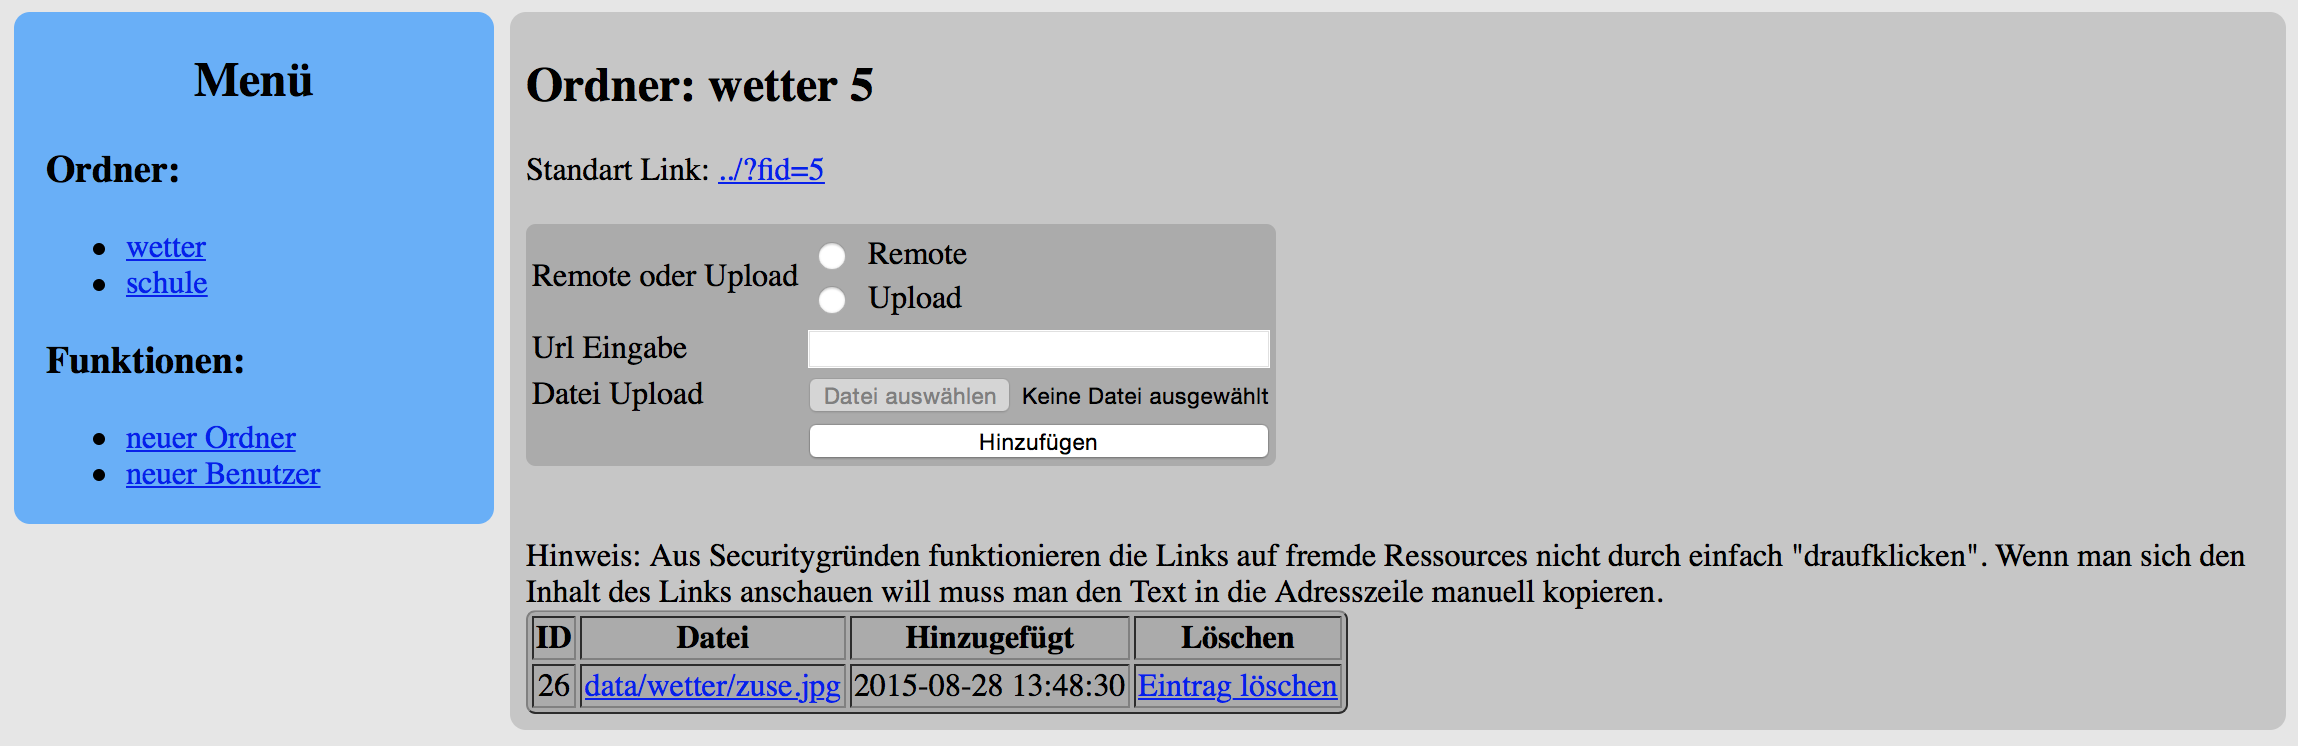
\includegraphics[width=\linewidth]{imgs/wms/wms_interface.png}
\end{center}

\subsection{Erreichbarkeit} % WMS
Auch wenn der Server nicht globales Interesse erweckt soll er natürlich nicht nur im Hafen erreichbar sein.
Da Standorte sich auch verändern können,
und nicht dringend immer in Kühlungsborn liegen müssen, ist der Server über den Domainnamen \link{http://wms.viwetter.de} erreichbar. \\
Alle Funktionen die hier beschrieben wurden sind demnach auch von jedem internetfähigen PC erreichbar. Keiner der Computer hat Sonderrechte,
und es werden auch keine Cookies gespeichert.

\subsection{Sicherheit} % WMS
Da dieses System an öffentlichen Orten Anwendung finden soll,
muss gewährleistet sein, dass auf den Anzeigegeräten nur Daten angezeigt werden,
die von autorisierten Personen ausgewählt worden.
Außerdem soll der Service nicht ohne unsere Erlaubnis und Wissen aufrufbar sein,
deshalb haben wir ein Kontensystem implementiert.
Da die Client Computer automatisiert starten und gleich die richtigen Daten anzeigen sollen,
mussten wir ein Protokoll entwickeln, welches sicher ist,
aber einem Rechner ermöglicht sich selbst einzuloggen.
